\section{WS6: Flying with network delay}
\label{section:ws6}
In this section the effects of network delay in when operating a swarm of drones is analysed. The results aim to show how the packet loss probability changes depending on interference, the number of drones flying at the same time and other factors.
\subsection{Setup of the test environment}
Before the flight begins it is ensured the radio addresses of the drones is the same as in the previous tests, namely "E7E7E7E701" for the "crazyflie1" and "E7E7E7E702" for "crazyflie2" Optitrack bodies. These values can be set by using the CrazyFlie Client as seen in Figure \ref{figure:crazyflie_client}.\\
\noindent As a next step the datarate of the CrazyRadio PA communication with the drones is changed from 2 Mbps to 250 kbps to more accurately reflect the TrueTime simulations in Section \ref{section:truetime}. The communication channel needs to be the same for all the drone in the swarm if they are to be controlled by the same Crazyradio PA\cite{book_ros}.\\

\noindent When choosing the channel it is important to select one that offers the least amount of interference. To measure the interference the "Link Quality" gauge from the Crazyflie Client can be examined.\\
\noindent The crazyflie can operate on 126 different Channels of 1MHz from 2400MHz to 2525MHz and the selected channel has to be in the 0-125 range\cite{web_crazyradio_wiki}. To avoid as much interference from other wireless networks as possible a network scanner app such as "Wifi Analyzer"\cite{web_wifi_analyzer_app} is used to see which channels are occupied. In the case of the lab where the test where conducted, channels up to 40 are occupied by other networks therefore channels 50 up to 125 are considered for the crazyflie swarm.\\

\noindent Switching the channel of the crazyflie shows little change in the "Link quality" gauge of the Crazyflie client therefore another method is needed. For this purpose the crazyflie ros stack offers an /rssi topic where the RSSI stands for "Received signal strength indication". To enable receiving data on that topic log messages from the drone have to be enabled by setting the \textit{enable\_logging} argument to \textit{True} i.e. in Listing \ref{listing:xml_multi_hover}. To test the rssi of a single drone, logging is enabled only for "crazyflie1" and the launch file is executed as usual:
\begin{mdframed}[backgroundcolor=light-gray, linecolor=light-gray]
\begin{verbatim}
$ roslaunch crazyflie_demo hover_multiple.launch
\end{verbatim}
\end{mdframed}

\noindent and in a separate terminal, display the RSSI data:

\begin{mdframed}[backgroundcolor=light-gray, linecolor=light-gray]
\begin{verbatim}
$ rosrun rqt_plot /crazyflie1/rssi
\end{verbatim}
\end{mdframed}

\noindent A new \texttt{rqt\_plot} window is opened as seen in Figure \ref{figure:rssi}
\begin{figure}[H]
\centering
 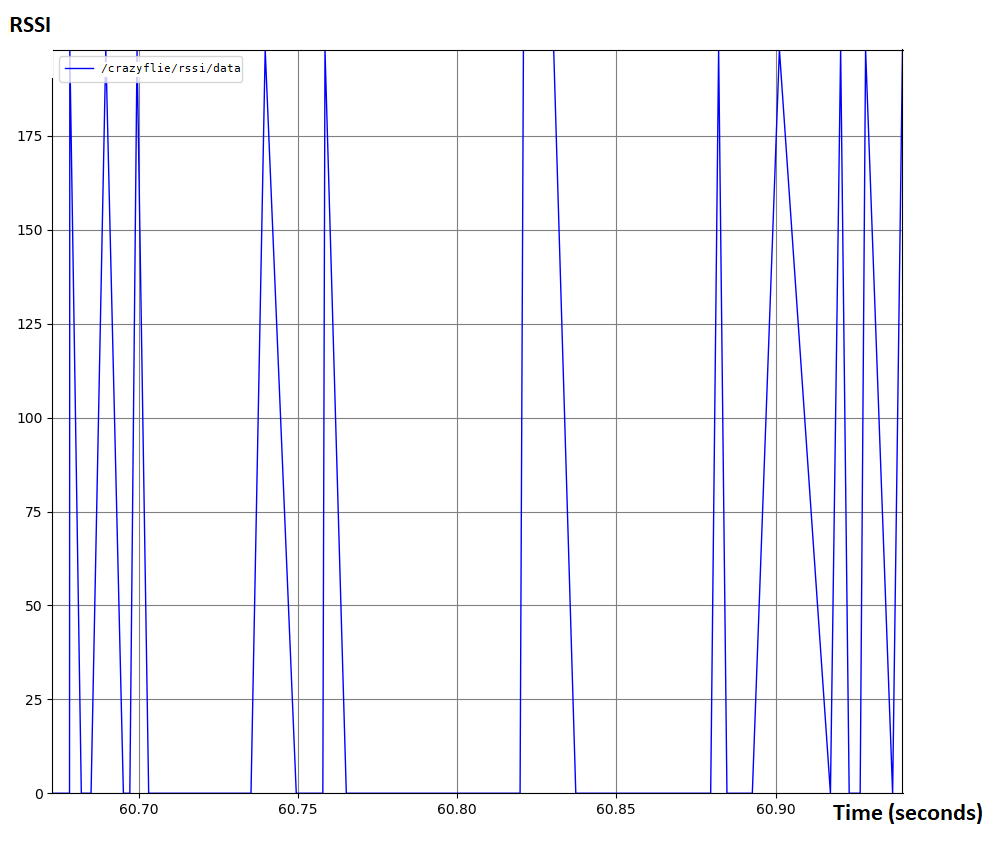
\includegraphics[scale=0.4]{Figures/rssi_data.png}
 \caption{rqt\_plot of the RSSI data}
 \label{figure:rssi}
\end{figure}

\noindent According to \cite{book_ros} an RSSI higher than 80 indicates increased interference on the wireless channel and another channel should be chosen. In Figure \ref{figure:rssi} the RSSI far exceeds this number if the crazyflie is set to channel 80. After trying multiple channels, channel 125 has been chosen as the one providing the better RSSI, ranging from 60 to 120, depending on the network activity. It is important to mention that it's not possible to receive any data on the \texttt{/rssi} topic when using 250 kpbs datarate, therefore 2 Mbps datarate has been chosen just for this test.\\

The last thing that needs to be done is to devise a way to simulate delayed packages when the drones are operational. It is found that the position controller relies upon the \textit{sendSetpoint()} function to send the setpoint to the internal controller of the Crazyflie. Therefore a delay is introduced in the function definition from the file located at \url{~/crazyflie_ws/src/crazyflie_ros/crazyflie_cpp/src/Crazyflie.cpp}

\begin{code}
\begin{minted}[breaklines, linenos, frame=single]{cpp}
void Crazyflie::sendSetpoint(
  float roll,
  float pitch,
  float yawrate,
  uint16_t thrust)
{
  crtpSetpointRequest request(roll, pitch, yawrate, thrust);
  // Sleep for a period of n milliseconds
  std::this_thread::sleep_for(std::chrono::milliseconds(20));
  sendPacket((const uint8_t*)&request, sizeof(request));
}
\end{minted}
\caption{A sleep time of n milliseconds is introduced in the function responsible for sending the reference point to the drones. In this case the reference setpoint calculated by the position controller arrives at the Crazyflie 20 ms later}
\label{listing:send_setpoint_delay}
\end{code}

\textbf{TODO: Code for publishing link quality}

This concludes the setup of the test environment. The next section discusses the flight behaviour of a drone swarm when network delay is present.

\subsection{Test flights}
For every performed test flight the link quality is plotted next to the position of the drones on the $z$-axis. The number of drones is set to two Crazyflie drones tracked by Optitrack. The drones are issued the takeoff command from the gamepad, left to fly for approximately 30 seconds after which they are requested to land. This type of test flight with no delay is shown is Figure \ref{figure:plot_hover_multiple}. The following figures show how the link quality and the flight behaviour of the drones changes as the delay time increases.

\begin{figure}[H]
\centering
 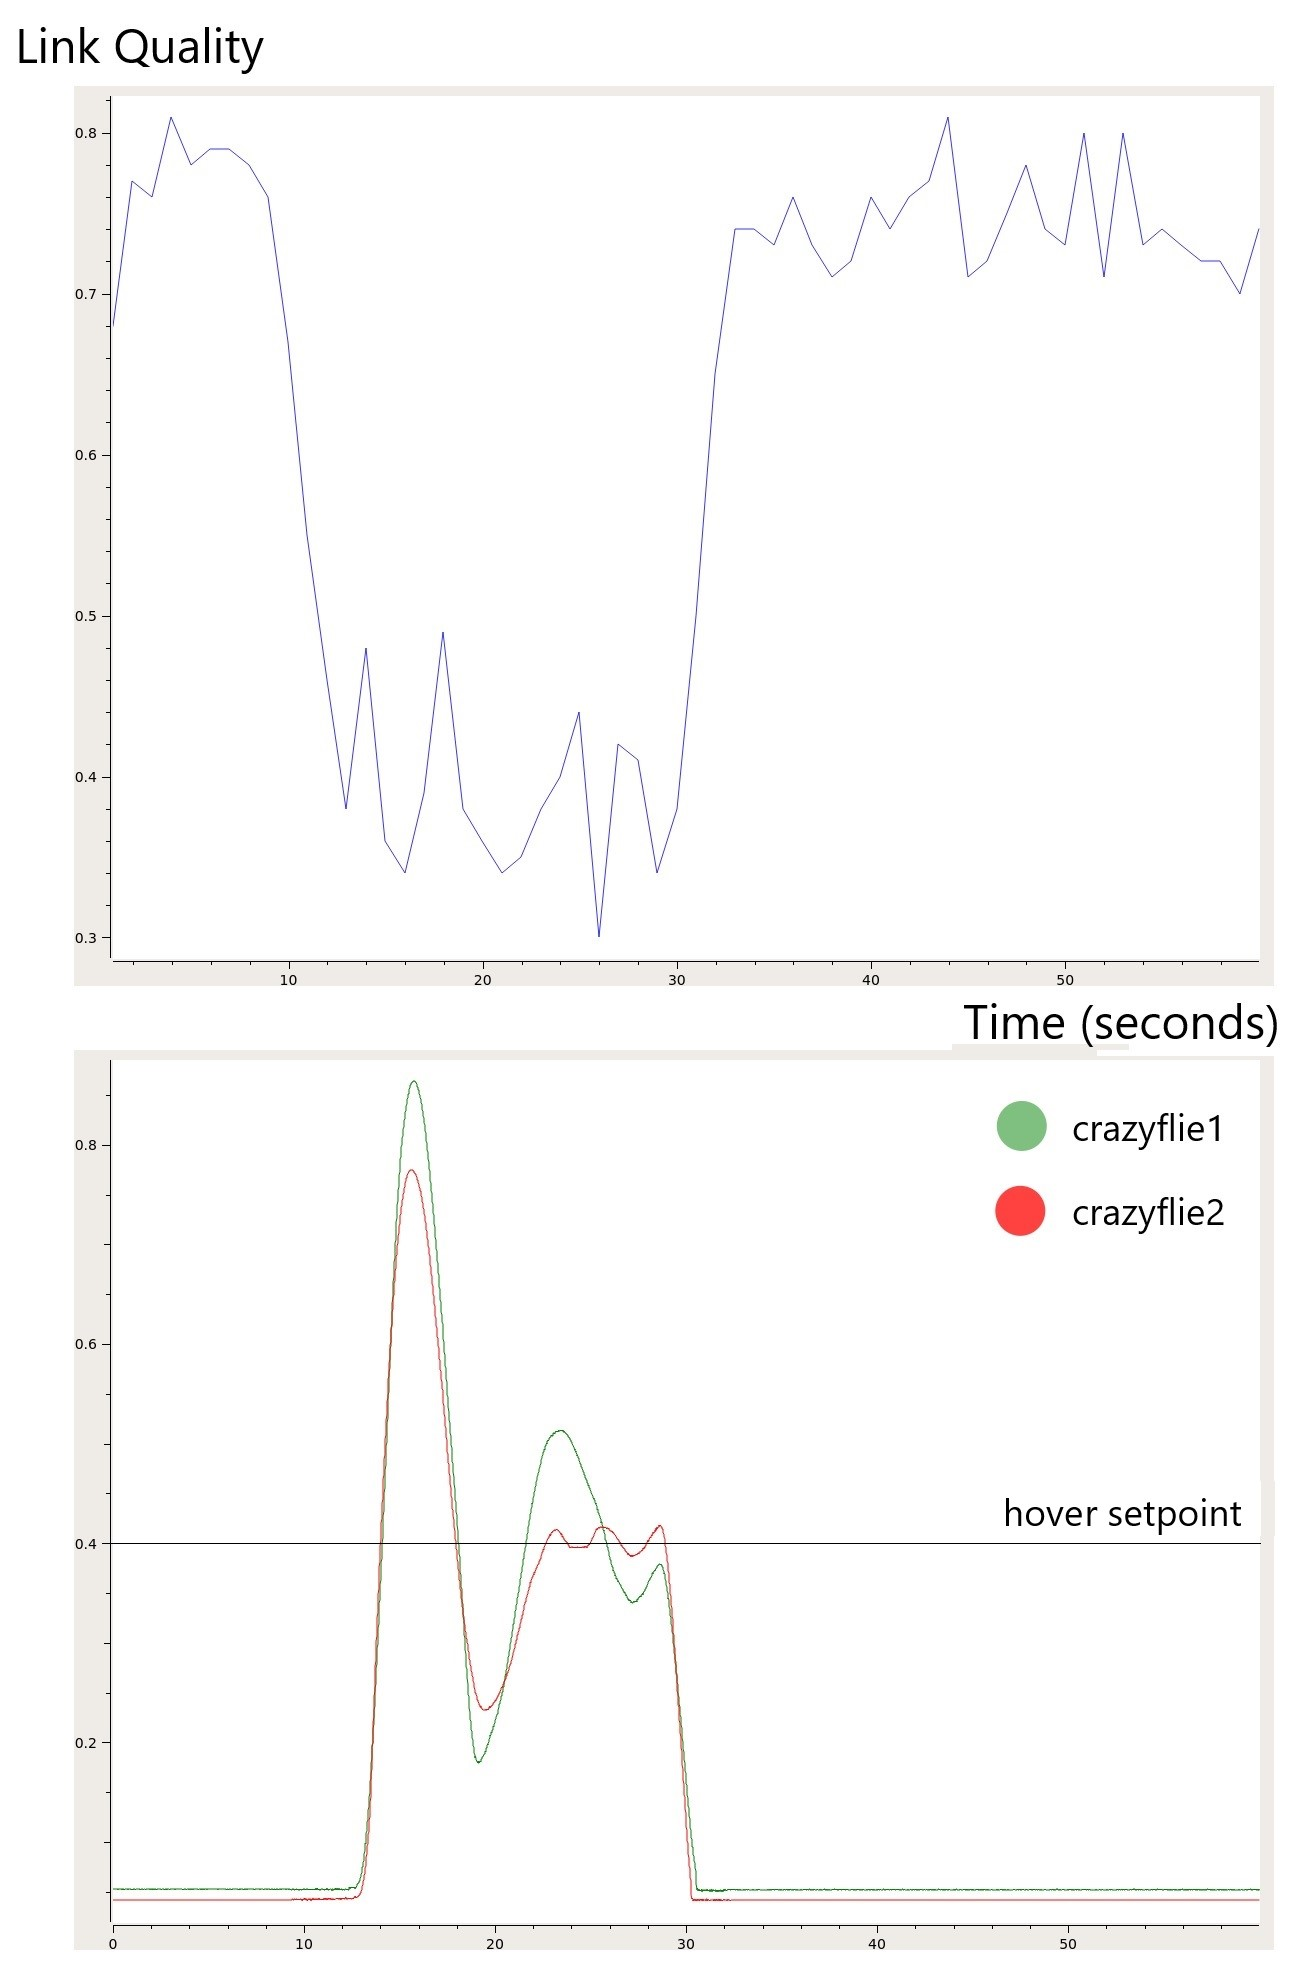
\includegraphics[scale=0.35]{Figures/delay_10.jpg}
 \caption{Delay 10}
 \label{figure:rssi}
\end{figure}

\noindent Up 10 ms delay the drones are able to takeoff and hover although with slight oscillations around the hover point instead of their $z$ position being almost equal as seen in Figure \ref{figure:plot_hover_multiple}

\begin{figure}[H]
\centering
 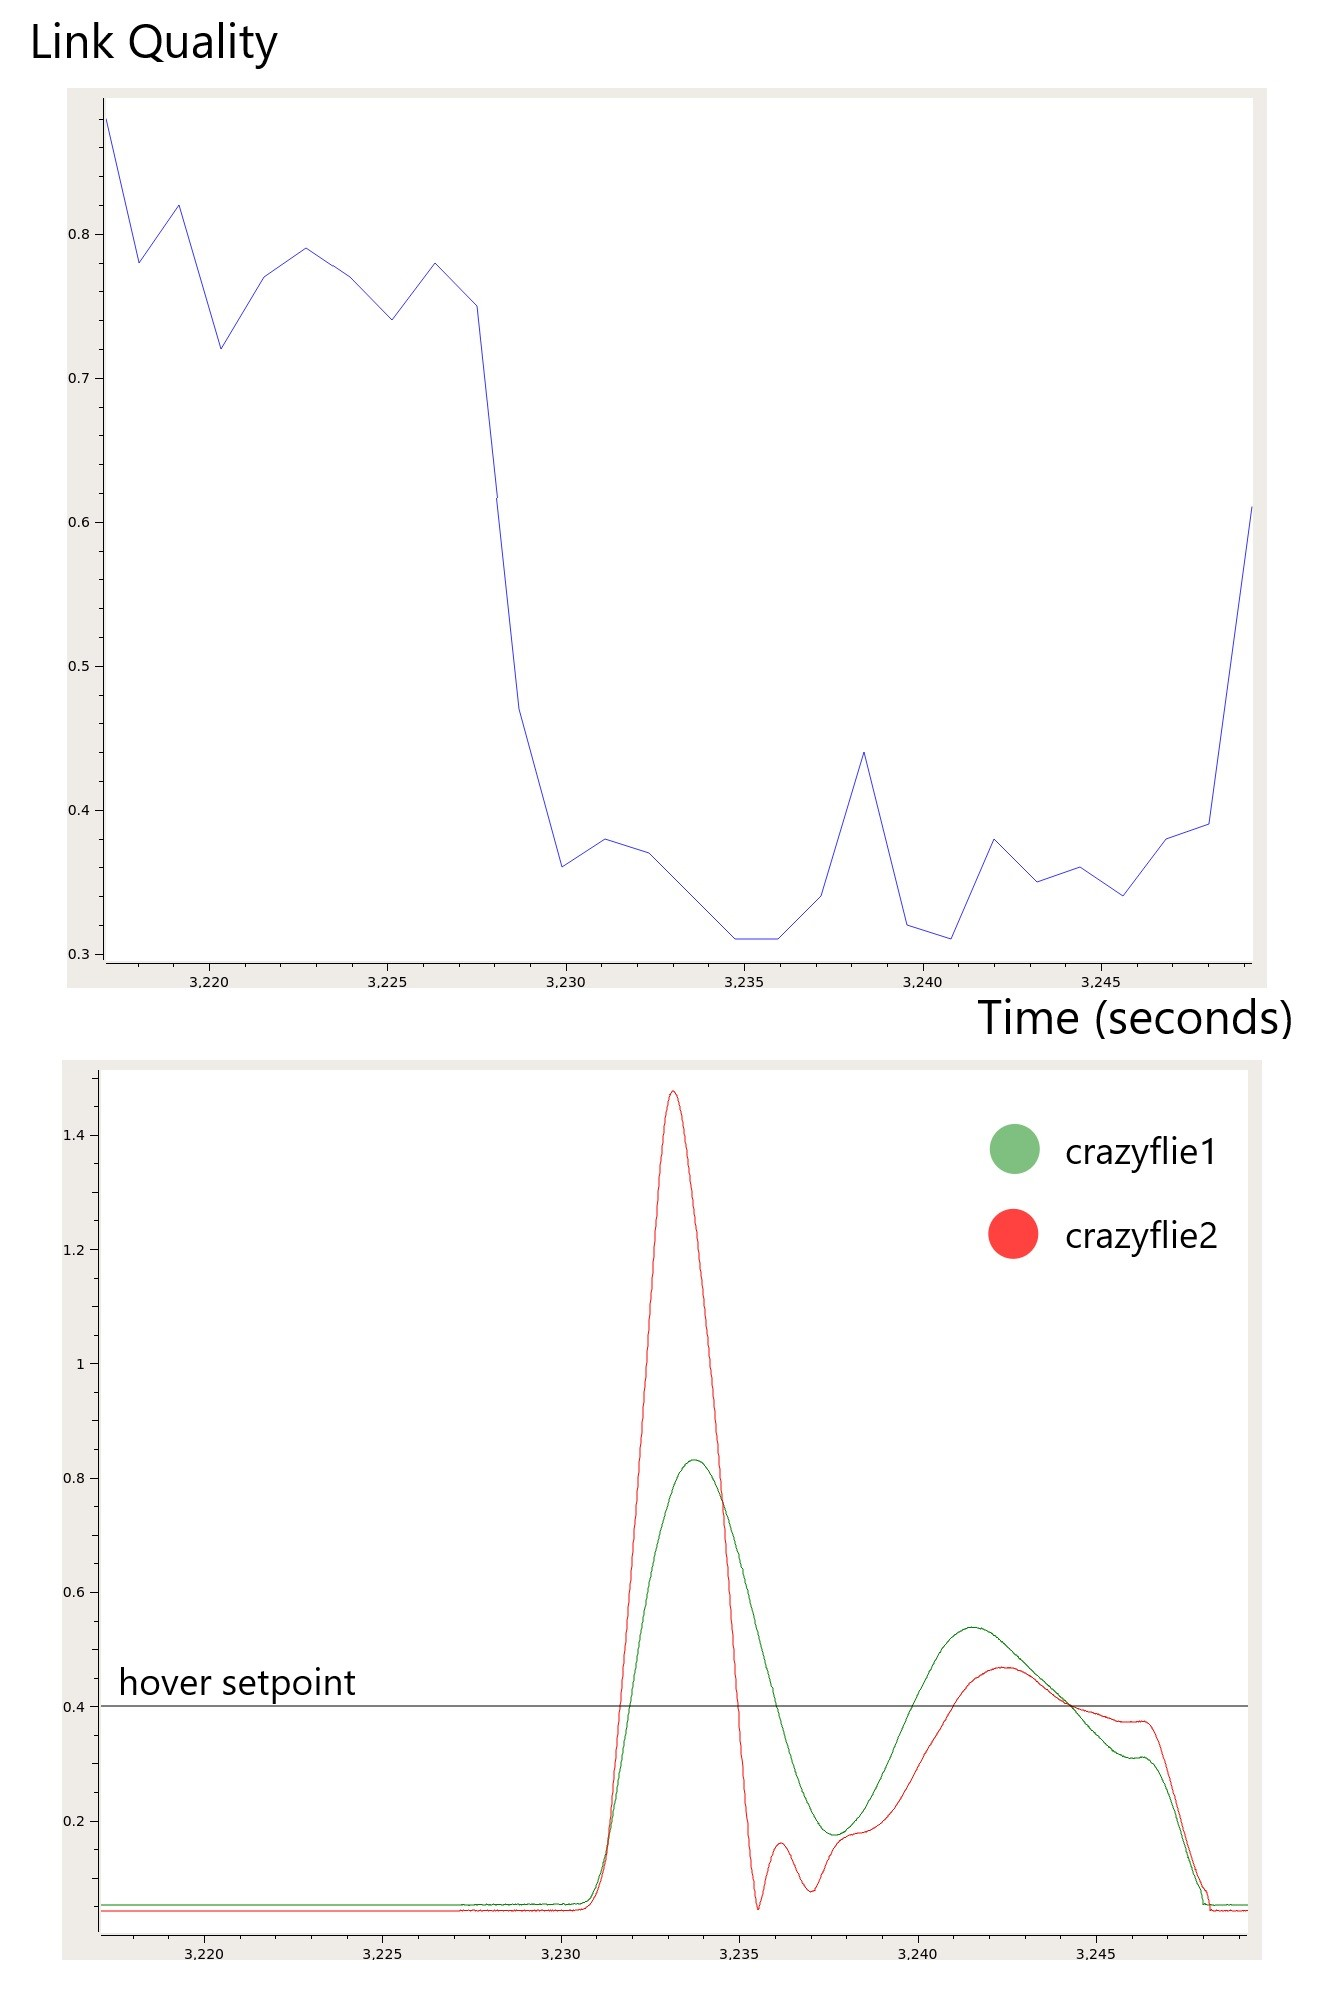
\includegraphics[scale=0.35]{Figures/delay_20.jpg}
 \caption{Delay 20}
 \label{figure:rssi}
\end{figure}

\noindent At 20 ms delaythere is a perceivable overshoot of crazyflie2 when taking off. Apart from the oscillations on the $z$ axis both drones are noticeably oscillating on the $x,y$ axes as well. For lower delays the drones are able to takeoff, hover and land even if they're a few centimetres off their starting position as defined in the launch file seen in Listing \ref{listing:xml_multi_hover}. For a delay of the ms, if the drones are not accurately on the starting position by a at most 5 centimetres they may exhibit unexpected behaviour such as suddenly flying out of bounds of the SmartCity layout. This also means that flights there is no guarantee that if a previous flight is successful the next one may not be.

\begin{figure}[H]
\centering
 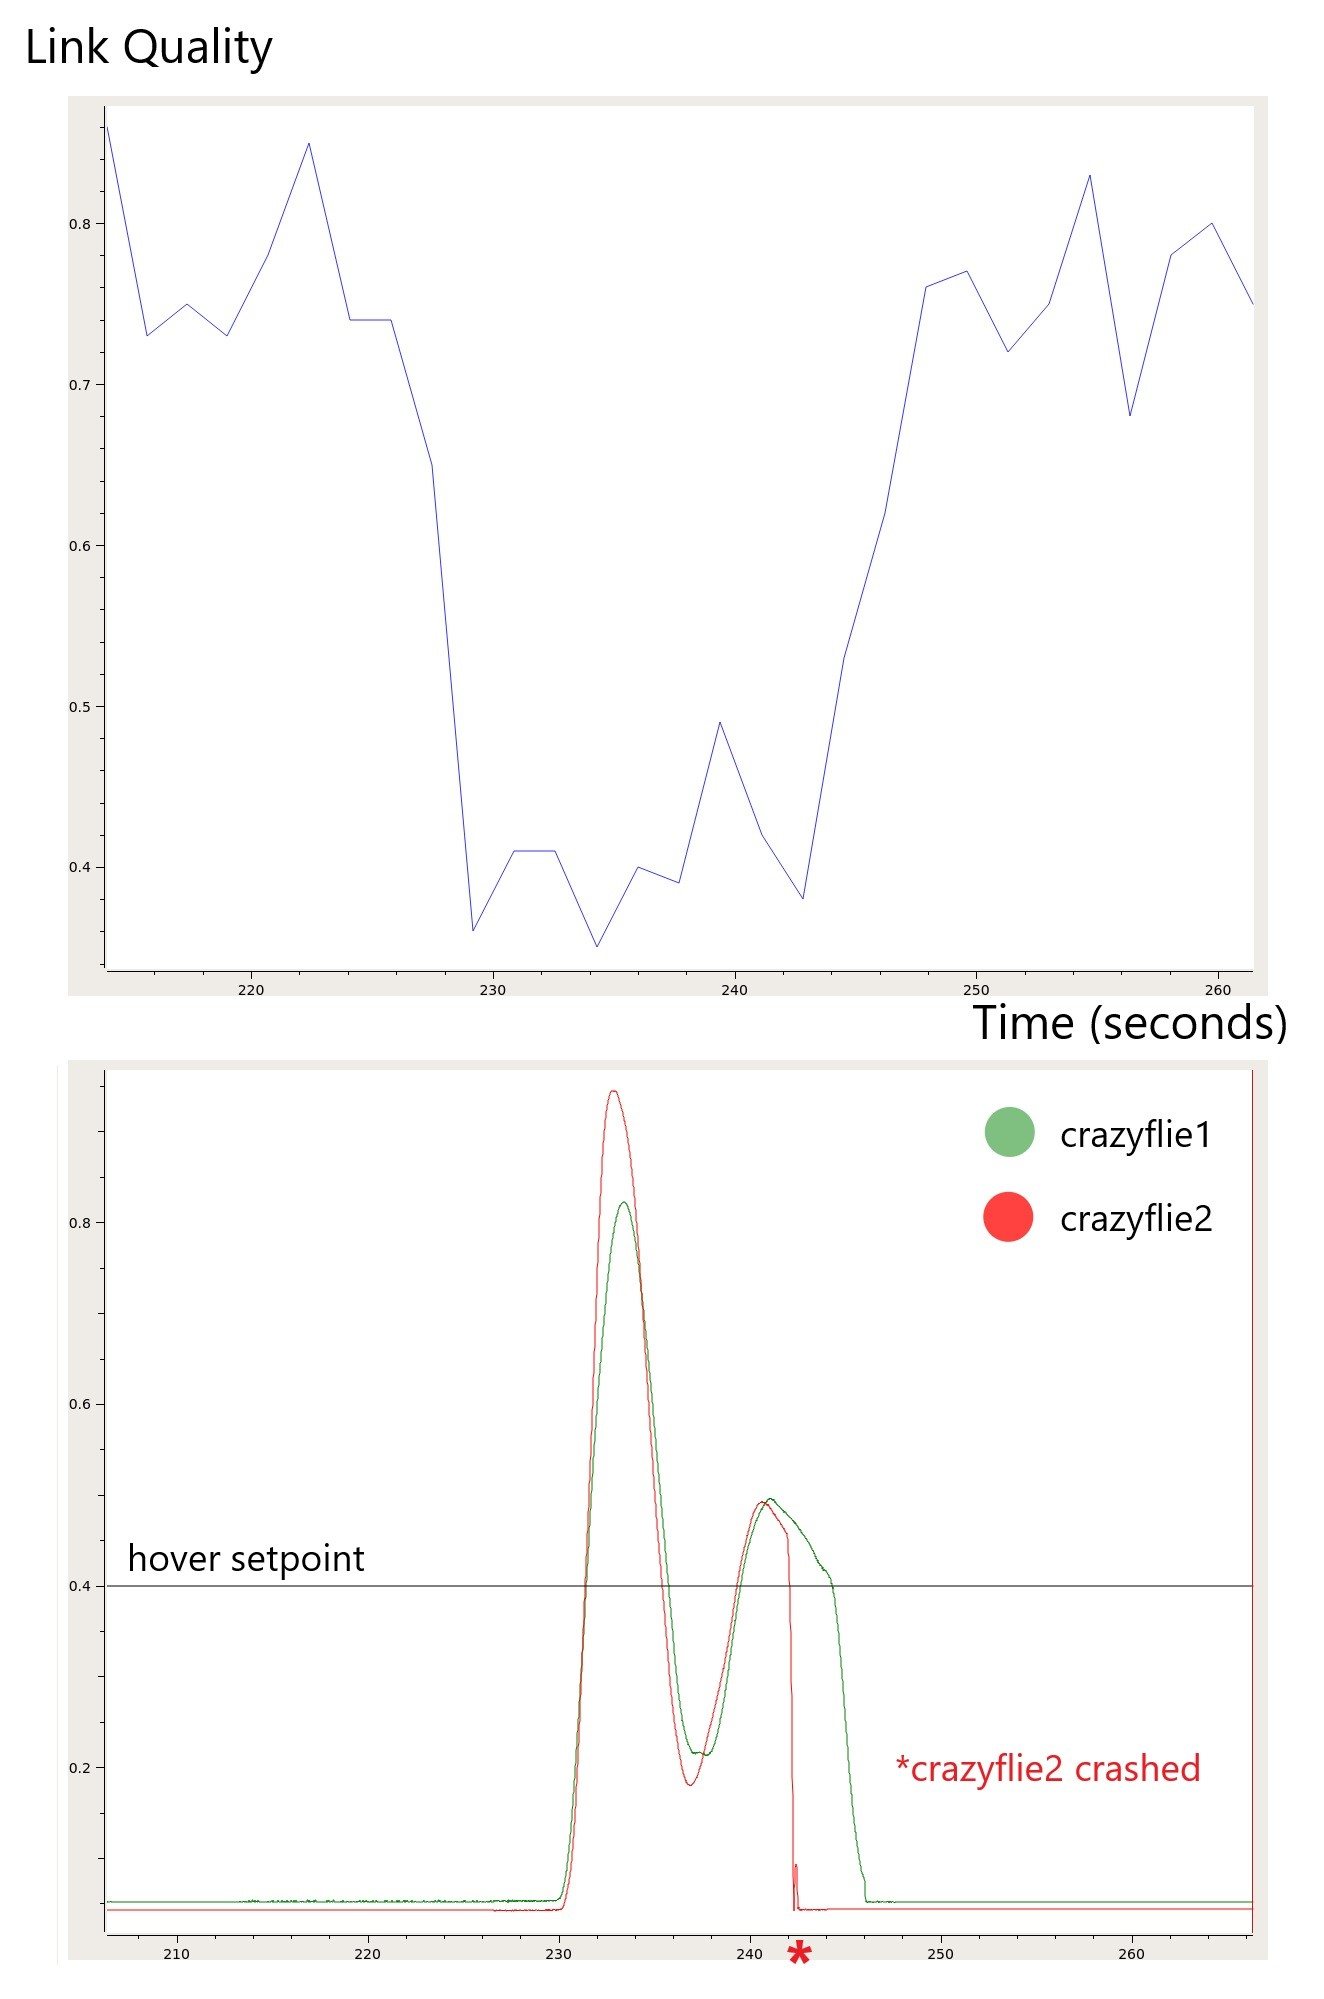
\includegraphics[scale=0.35]{Figures/delay_30.jpg}
 \caption{Delay 30}
 \label{figure:rssi}
\end{figure}

\noindent At a delay of 30 ms the drones are unpredictable most of the time. In the figure above the crazyflie2 drone droppped on the ground without being issued the landing command. Successful flights can still be achieved by having the drones' starting point accurate to 5 centimetres to what is in the launch file but the successful flight probability is lesser than on 20 ms delay.